% Hierarchy of process classes, by the resources needed to generate them.
% Editable replacement for the hierarchy.png raster.
  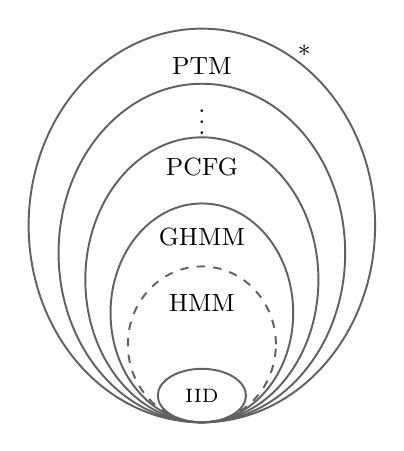
\begin{tikzpicture}[
    ring/.style={draw=black!62,line width=.7pt},
    ghmm/.style={fill=green!62},
    growth/.style={-{Stealth[length=1.6mm,width=1.4mm]},green!60!black,line width=.6pt},
  ]
    % Each class is an oval sitting on a common bottom point at the origin, so
    % containment reads off the nesting: IID inside HMM inside GHMM, and so on.
    \draw[ring] (0,2.50) ellipse[x radius=2.20, y radius=2.50];
    \draw[ring] (0,2.15) ellipse[x radius=1.82, y radius=2.15];
    \draw[ring] (0,1.81) ellipse[x radius=1.48, y radius=1.81];
    \draw[ring] (0,1.39) ellipse[x radius=1.16, y radius=1.39];
    \draw[ring,dashed] (0,0.99) ellipse[x radius=0.94, y radius=0.99];
    \draw[ring] (0,0.34) ellipse[x radius=0.56, y radius=0.34];
    \node[font=\small] at (0,4.52) {PTM};
    \node[font=\small] at (0,3.92) {$\vdots$};
    \node[font=\small] at (0,3.24) {PCFG};
    \node[font=\small] at (0,2.36) {GHMM};
    \node[font=\small] at (0,1.52) {HMM};
    \node[font=\scriptsize] at (0,0.34) {IID};
    \node[font=\small] at (1.30,4.72) {$*$};  % see "not exhaustive"
  \end{tikzpicture}
